\subsection{UC6 - Consultazione di una prenotazione da parte dell'amministratore}\label{usecase:6}
\begin{figure}[H]
  \centering
  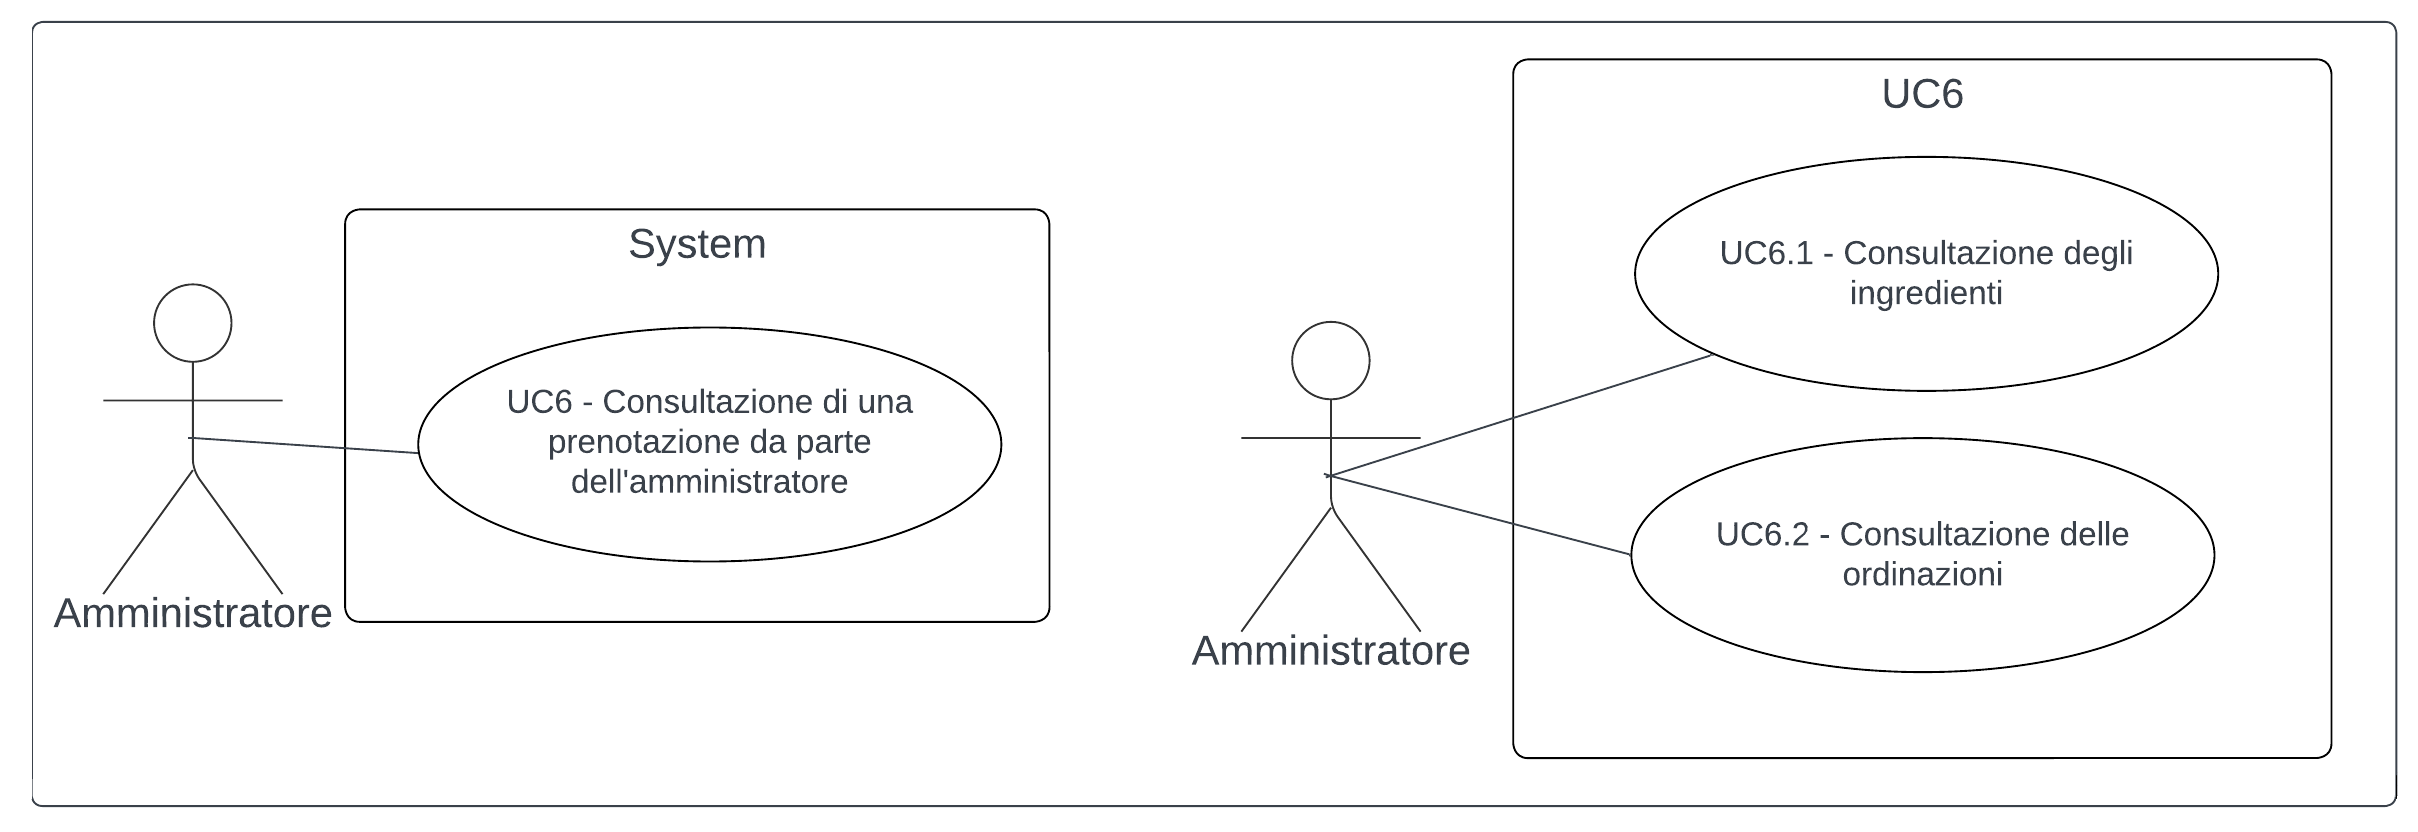
\includegraphics[width=1\textwidth]{ucd/UCD6_new.png}
\end{figure}
\textbf{Attori}:
\begin{itemize}
    \item Amministratore
\end{itemize}
\textbf{Precondizioni}:
\begin{itemize}
    \item L'amministratore in fase di registrazione ha inserito un ristorante di cui poter consultare le prenotazioni
    \item L'amministratore visualizza le prenotazioni dalla lista delle prenotazioni (\nameref{usecase:15})
\end{itemize}
\textbf{Postcondizioni}:
\begin{itemize}
    \item L'amministratore visualizza nel dettaglio le informazioni di una prenotazione
\end{itemize}
\textbf{Scenario principale}:
\begin{enumerate}
    \item L'utente visualizza le informazioni di una singola $\textit{Prenotazione}_G$ effettuata, tra cui:
    \begin{enumerate}
        \item gli ingredienti necessari per quella $\textit{Prenotazione}_G$ (\nameref{usecase:6_1})
        \item le ordinazioni associate a quella prenotazione
        (\nameref{usecase:6_2})
    \end{enumerate}
\end{enumerate}